\documentclass[aspectratio=169]{beamer}
\usetheme{Madrid}
\usecolortheme{default}

% Remove navigation symbols and footer
\setbeamertemplate{navigation symbols}{}
\setbeamertemplate{footline}{}

% Packages
\usepackage{graphicx}
\usepackage{booktabs}
\usepackage{amsmath}
\usepackage{tikz}
\usepackage{listings}
\usepackage{xcolor}
\usepackage{hyperref}
\usepackage{multicol}

% Custom colors
\definecolor{darkblue}{RGB}{0,51,102}
\definecolor{lightblue}{RGB}{102,178,255}
\definecolor{codegreen}{rgb}{0,0.6,0}
\definecolor{codegray}{rgb}{0.5,0.5,0.5}
\definecolor{codepurple}{rgb}{0.58,0,0.82}

% Code styling
\lstset{
    basicstyle=\ttfamily\tiny,
    keywordstyle=\color{blue},
    commentstyle=\color{codegreen},
    stringstyle=\color{codepurple},
    numberstyle=\tiny\color{codegray},
    breaklines=true,
    showstringspaces=false,
    columns=flexible,
    keepspaces=true,
    literate={-}{-}1
}

% Title page information
\title[Music Genre Discovery]{Unsupervised Music Genre Discovery Using Audio Feature Learning}
\subtitle{A Comprehensive Multi-Dataset Analysis}
\author{Anirudh Sharma \\ Roll No.: 22dcs002}
\institute[NIT Hamirpur]{
    Department of Computer Science and Engineering \\
    National Institute of Technology Hamirpur \\
    \vspace{0.3cm}
    Machine Learning Assignment (CS-652) \\
    Semester-7 (2025)
}
\date{} % Remove date

\begin{document}

% Clean and Compact Title Slide (no background, fits perfectly)
\begin{frame}[plain]
    \begin{center}
        \vspace*{0.5cm}

        % --- Main Title ---
        {\LARGE \textbf{Unsupervised Music Genre Discovery}}\\[0.2cm]
        {\Large \textbf{Using Audio Feature Learning}}\\[0.3cm]

        % --- Logo (centered, optional placeholder) ---
        \IfFileExists{images/nith_logo.png}{
            \includegraphics[width=0.17\textwidth]{images/nith_logo.png}
        }{
            \fbox{\parbox{0.17\textwidth}{\centering NITH\\Logo}}
        }\\[0.5cm]

        % --- Institute Info ---
        {\small Department of Computer Science and Engineering}\\
        {\small \textbf{National Institute of Technology Hamirpur}}\\[0.5cm]

        % --- Author Info ---
        {\normalsize \textbf{Anirudh Sharma}}\\
        {\small Roll No.: 22dcs002}\\[0.2cm]

        % --- Course Info ---
        {\footnotesize Machine Learning Assignment (CS-652)}
    \end{center}
\end{frame}


% Table of Contents
\begin{frame}{Table of Contents}
    \tableofcontents
\end{frame}

% Section 1: Introduction
\section{Introduction}

\begin{frame}{Introduction}
    \frametitle{Unsupervised Music Genre Discovery using Audio Feature Learning}
    
    \begin{block}{Overview}
        \begin{itemize}
            \item The explosion of digital music platforms has led to massive unlabelled music data
            \item Manual genre tagging is subjective, inconsistent, and time-consuming
            \item This project aims to automatically discover and cluster music genres using unsupervised learning techniques
        \end{itemize}
    \end{block}
    
    \begin{block}{Problem Statement}
        \textbf{How can we identify underlying genre patterns and clusters in diverse music datasets without labeled data?}
    \end{block}
\end{frame}

\begin{frame}{Objectives}
    \begin{enumerate}
        \item Extract meaningful audio and metadata features (MFCC, Spectral, Chroma, Tempo, etc.)
        \item Apply unsupervised learning algorithms to discover natural groupings of songs
        \item Compare performance across multiple datasets and evaluation metrics
        \item Visualize cluster separability and interpret genre similarities
    \end{enumerate}
    
    \vspace{0.5cm}
    
    \begin{block}{Expected Outcome}
        \begin{itemize}
            \item Discover genre clusters without supervision
            \item Identify feature patterns that separate musical styles
            \item Evaluate which algorithm and dataset combination yields the best clustering quality
        \end{itemize}
    \end{block}
\end{frame}

% Section 5: Tech Stack
\section{Implementation}

\begin{frame}{Technology Stack}
    \begin{columns}
        \column{0.5\textwidth}
        \textbf{Core Libraries}
        \begin{itemize}
            \item \textbf{Librosa}: Audio feature extraction
            \item \textbf{Scikit-learn}: ML algorithms
            \item \textbf{NumPy/Pandas}: Data manipulation
            \item \textbf{Matplotlib/Seaborn}: Visualization
        \end{itemize}
        
        \vspace{0.3cm}
        
        \textbf{Platforms \& Tools}
        \begin{itemize}
            \item \textbf{Kaggle}: Dataset access \& compute
            \item \textbf{Weights \& Biases}: Experiment tracking
            \item \textbf{Jupyter}: Interactive development
        \end{itemize}
        
        \column{0.5\textwidth}
        \begin{center}
            \Large
            \textbf{Tech Stack}
            
            \vspace{0.5cm}
            
            \begin{itemize}
                \item[$\checkmark$] Python 3.8+
                \item[$\checkmark$] Librosa
                \item[$\checkmark$] Scikit-learn
                \item[$\checkmark$] K-Means / DBSCAN / GMM
                \item[$\checkmark$] PCA / t-SNE
                \item[$\checkmark$] Kaggle Notebooks
                \item[$\checkmark$] WandB.ai
            \end{itemize}
        \end{center}
    \end{columns}
\end{frame}


% Section 4: Methodology
\section{Methodology}

\begin{frame}{Methodology Overview}
    \framesubtitle{Complete Pipeline}
    
    \begin{center}
        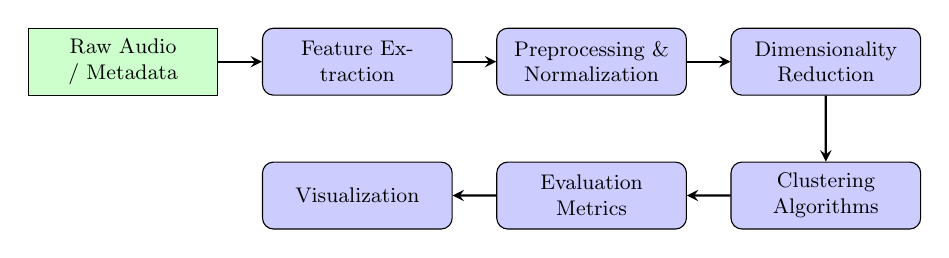
\begin{tikzpicture}[scale=0.85, every node/.style={transform shape}]
            % Define styles
            \tikzstyle{process} = [rectangle, rounded corners, minimum width=2.8cm, minimum height=1cm, text centered, draw=black, fill=blue!20, font=\small, text width=2.6cm]
            \tikzstyle{data} = [rectangle, minimum width=2.8cm, minimum height=1cm, text centered, draw=black, fill=green!20, font=\small, text width=2.6cm]
            \tikzstyle{arrow} = [thick,->,>=stealth]
            
            % First row - horizontal (left to right)
            \node (data) [data] at (0,0) {Raw Audio / Metadata};
            \node (extract) [process] at (3.5,0) {Feature Extraction};
            \node (preprocess) [process] at (7,0) {Preprocessing \& Normalization};
            
            % Arrow connecting to second row
            \node (reduce) [process] at (10.5,0) {Dimensionality Reduction};
            
            % Second row - horizontal (right to left)
            \node (cluster) [process] at (10.5,-2) {Clustering Algorithms};
            \node (evaluate) [process] at (7,-2) {Evaluation Metrics};
            
            % Third row - centered
            \node (visualize) [process] at (3.5,-2) {Visualization};
            
            % Arrows - horizontal flow, then down, then back
            \draw [arrow] (data) -- (extract);
            \draw [arrow] (extract) -- (preprocess);
            \draw [arrow] (preprocess) -- (reduce);
            \draw [arrow] (reduce) -- (cluster);
            \draw [arrow] (cluster) -- (evaluate);
            \draw [arrow] (evaluate) -- (visualize);
        \end{tikzpicture}
    \end{center}
\end{frame}

% Section 2: Audio Features
\section{Audio Feature Extraction}

\begin{frame}{Audio Feature Extraction}
    
    \begin{block}{Feature Extraction Overview}
        We extract time and frequency domain features from audio files for classification:
        \begin{itemize}
            \item \textbf{Temporal Features}: Zero-crossing rate, Energy, Pitch
            \item \textbf{Spectral Features}: Spectral centroids, Spectral Roll-off, Spectral Flux, Spectral Entropy
            \item \textbf{Time-Frequency Features}: Spectrograms, Mel-spectrograms, MFCC, Chromagrams
        \end{itemize}
    \end{block}
    
    \begin{alertblock}{Classification Challenge}
        Some genres are highly similar and overlap significantly:
        \begin{itemize}
            \item Country vs. Rock
            \item Pop vs. Disco
            \item Jazz vs. Reggae
        \end{itemize}
        Features like spectrograms and MFCCs contain both time and frequency information, making them powerful for distinguishing genres.
    \end{alertblock}
\end{frame}

% \begin{frame}[fragile]{1. Spectrogram}
    
%     \begin{columns}
%         \column{0.45\textwidth}
%         \textbf{What is a Spectrogram?}
%         \begin{itemize}
%             \item Visual representation of signal strength over time
%             \item Also known as sonographs or voicegrams
%             \item \textbf{Three dimensions}:
%             \begin{itemize}
%                 \item \textcolor{blue}{Time (x-axis)}
%                 \item \textcolor{red}{Frequency (y-axis)}
%                 \item \textcolor{orange}{Amplitude (color)}
%             \end{itemize}
%         \end{itemize}
        
%         \vspace{0.2cm}
        
%         \textbf{How it's computed?}
%         \begin{itemize}
%             \item Audio segmented into overlapping windows
%             \item Short-Time Fourier Transform (STFT)
%             \item Squared magnitude computed
%             % \item Windows placed side-by-side
%         \end{itemize}
        
%         \column{0.55\textwidth}
%         \begin{center}
%             \includegraphics[width=\textwidth]{images/Spectrogram.png}
            
%             \vspace{0.3cm}
            
%             \tiny
%             \textit{Spectrogram showing frequency content over time}
%         \end{center}
        
%         \vspace{0.3cm}
        
%         \begin{block}{Key Insight}
%             \small
%             Spectrograms reveal the complete frequency content of audio as it evolves over time
%         \end{block}
%     \end{columns}
% \end{frame}


% \begin{frame}[fragile]{2. Mel-Spectrogram}
    
%     \begin{columns}
%         \column{0.45\textwidth}
%         \textbf{What is Mel-Spectrogram?}
%         \begin{itemize}
%             \item \textbf{Mel scale}: Perceptual pitch scale
%             \item Humans detect lower frequencies better
%             \item Example: 200Hz vs 400Hz (easy) \\ 2000Hz vs 2200Hz (hard)
%             \item Groups higher frequencies exponentially
%         \end{itemize}
        
%         \vspace{0.2cm}
        
%         \textbf{How it's computed?}
%         \begin{itemize}
%             \item Start with spectrogram
%             \item Apply mel filter-banks
%             \item Map frequency to mel scale
%         \end{itemize}
        
%         \vspace{0.2cm}
        
        
        
%         \column{0.55\textwidth}
%         \begin{center}
%             \includegraphics[width=\textwidth]{images/Mel_spectrogram.png}
            
%             \vspace{0.3cm}
            
%             \tiny
%             \textit{Mel-Spectrogram with perceptual frequency scale}
%         \end{center}
        
%         \vspace{0.2cm}
        
%         \begin{lstlisting}[language=Python]
% # Compute Mel-Spectrogram
% mel_spec = librosa.feature.melspectrogram(
%     y=y, 
%     sr=sr,
%     n_fft=2048,
%     hop_length=512,
%     n_mels=128
% )

% # Convert to dB
% mel_spec_db = librosa.power_to_db(
%     mel_spec, 
%     ref=np.max
% )
%         \end{lstlisting}
% \begin{block}{Processing}
%             \small
%             Audio $\rightarrow$ Spectrogram $\rightarrow$ Mel Filter $\rightarrow$ Mel-Spec
%         \end{block}
%     \end{columns}
% \end{frame}

% \begin{frame}[fragile]{3. MFCC (Mel-Frequency Cepstral Coefficients)}
    
%     \begin{columns}
%         \column{0.45\textwidth}
%         \textbf{What is MFCC?}
%         \begin{itemize}
%             \item Compact representation of spectral envelope
%             \item Uses Mel scale + DCT
%             \item Compresses Mel-Spectrogram data
%             \item Represents vocal tract shape
%             \item \textbf{Most important} for genre classification
%         \end{itemize}
        
%         \vspace{0.2cm}
        
%         \textbf{Processing Pipeline}
%         \begin{enumerate}
%             \item Compute Mel-Spectrogram
%             \item Apply Discrete Cosine Transform (DCT)
%             \item Extract first 13-20 coefficients
%             \item Compute mean \& variance
%         \end{enumerate}
        
%         \column{0.55\textwidth}
%         \begin{center}
%             \includegraphics[width=\textwidth]{images/MFCC.png}
            
%             \vspace{0.3cm}
            
%             \tiny
%             \textit{MFCC coefficients showing timbral characteristics}
%         \end{center}
        
%         \vspace{0.2cm}
        
%         \begin{lstlisting}[language=Python]
% # Extract MFCC coefficients
% mfccs = librosa.feature.mfcc(
%     y=y, 
%     sr=sr,
%     n_mfcc=20,
%     n_fft=2048,
%     hop_length=512
% )

% # Compute statistics
% mfcc_mean = np.mean(mfccs, axis=1)
% mfcc_var = np.var(mfccs, axis=1)

% # Total: 40 features (20 mean + 20 var)
%         \end{lstlisting}
%     \end{columns}
% \end{frame}

\begin{frame}{Complete Feature Extraction Pipeline}
    
    \begin{columns}
        \column{0.55\textwidth}
        \textbf{Features Extracted Per Audio File}
        
        \vspace{0.3cm}
        
        \begin{table}[h]
            \centering
            \small
            \begin{tabular}{lcp{3.5cm}}
                \toprule
                \textbf{Feature} & \textbf{Count} & \textbf{Description} \\
                \midrule
                \textbf{MFCCs} & 40 & 20 coeffs (mean \& var) \\
                \midrule
                \textbf{Spectral} & 6 & Centroid, BW, Rolloff \\
                \midrule
                \textbf{Chroma} & 2 & 12 pitch classes \\
                \midrule
                \textbf{Temporal} & 4 & ZCR, RMS Energy \\
                \midrule
                \textbf{Rhythmic} & 1 & Tempo (BPM) \\
                \midrule
                \textbf{Harmonic} & 5 & Harmony, Perceptr \\
                \midrule
                \textbf{Total} & \textbf{58} & Complete vector \\
                \bottomrule
            \end{tabular}
        \end{table}
        
        \column{0.45\textwidth}
        \begin{alertblock}{Why MFCC Dominates?}
            \small
            \begin{itemize}
                \item \textbf{Compact}: 40/58 features (69\%)
                \item \textbf{Perceptual}: Matches human hearing
                \item \textbf{Discriminative}: Best genre separation
                \item \textbf{Efficient}: Compressed spectral envelope
            \end{itemize}
        \end{alertblock}
        
        \vspace{0.3cm}
        
        \begin{block}{Feature Statistics}
            \small
            \begin{itemize}
                \item Mean \& variance computed
                \item Aggregated over time
                \item Normalized for clustering
                \item 58-dimensional feature vector
            \end{itemize}
        \end{block}
    \end{columns}
\end{frame}

\begin{frame}[fragile]{Feature Extraction Methods}
    \begin{columns}
        \column{0.5\textwidth}
        \textbf{Audio Feature Extraction}
        \begin{itemize}
            \item \textbf{Library}: Librosa (Python)
            \item Window size: 2048 samples
            \item Hop length: 512 samples
            \item Sample rate: 22050 Hz
            \item Aggregate: mean \& variance
        \end{itemize}
        
        \vspace{0.3cm}
        
        \textbf{Metadata Features}
        \begin{itemize}
            \item Spotify API for semantic features
            \item Pre-computed features from datasets
        \end{itemize}
        
        \column{0.5\textwidth}
        \begin{lstlisting}[language=Python]
import librosa

# Load audio
y, sr = librosa.load(audio_file)

# Extract features
mfccs = librosa.feature.mfcc(y, sr, n_mfcc=20)
chroma = librosa.feature.chroma_stft(y, sr)
spec_cent = librosa.feature.spectral_centroid(y, sr)
zcr = librosa.feature.zero_crossing_rate(y)
tempo, _ = librosa.beat.beat_track(y, sr)

# Aggregate
features = {
    'mfcc_mean': np.mean(mfccs, axis=1),
    'mfcc_var': np.var(mfccs, axis=1),
    ...
}
        \end{lstlisting}
    \end{columns}
\end{frame}

% Section 3: Datasets
\section{Datasets}

\begin{frame}{Datasets Overview}
    
    \begin{table}[h]
        \centering
        \small
        \begin{tabular}{lcccc}
            \toprule
            \textbf{Dataset} & \textbf{Size} & \textbf{Format} & \textbf{Features} & \textbf{Genres} \\
            \midrule
            \textbf{GTZAN} & 1,000 & MP3 (30s) & 58 & 10 \\
            \textbf{FMA} & 8,000 & WAV (30s) & 160 & 8 \\
            \textbf{MSD} & 10,000 & HDF5 & 90 & Unknown \\
            \textbf{Spotify} & 170K+ & Metadata & 18 & Unknown \\
            \bottomrule
        \end{tabular}
    \end{table}
    
    \vspace{0.3cm}
    
    \begin{columns}
        \column{0.5\textwidth}
        \textbf{Audio-Based Datasets}
        \begin{itemize}
            \item GTZAN: Pre-extracted features
            \item FMA: Raw audio + extraction
            \item MSD: Million Song subset
        \end{itemize}
        
        \column{0.5\textwidth}
        \textbf{Metadata-Based}
        \begin{itemize}
            \item Spotify: API features
            \item Valence, energy, danceability
            \item Acoustic \& instrumental
        \end{itemize}
    \end{columns}
\end{frame}

\begin{frame}{Dataset 1: GTZAN Music Genre Dataset}
    
    \begin{columns}
        \column{0.5\textwidth}
        \textbf{Dataset Characteristics}
        \begin{itemize}
            \item \textbf{Source}: 1,000 audio tracks (30s each)
            \item \textbf{Format}: MP3, pre-extracted features
            \item \textbf{Genres}: 10 (100 songs each)
            \begin{itemize}
                \footnotesize
                \item Blues, Classical, Country
                \item Disco, Hip-hop, Jazz
                \item Metal, Pop, Reggae, Rock
            \end{itemize}
            \item \textbf{Features}: 58 total
        \end{itemize}
        
        \vspace{0.3cm}
        
        \textbf{Reference}
        \begin{itemize}
            \item G. Tzanetakis \& P. Cook (2002)
            \item IEEE Trans. Speech \& Audio
        \end{itemize}
        
        \column{0.5\textwidth}
        \textbf{Feature Breakdown}
        \begin{itemize}
            \item \textbf{MFCCs}: 20 coefficients (mean \& var)
            \item \textbf{Spectral}: 6 features
            \begin{itemize}
                \footnotesize
                \item Centroid, Bandwidth
                \item Rolloff, Contrast
            \end{itemize}
            \item \textbf{Chroma}: 12 (mean \& var)
            \item \textbf{Temporal}: ZCR, RMS
            \item \textbf{Harmonic}: Harmony, Perceptr
            \item \textbf{Rhythmic}: Tempo (BPM)
        \end{itemize}
        
        \vspace{0.2cm}
        
        \begin{alertblock}{Techniques Used}
            \footnotesize
            StandardScaler $\rightarrow$ PCA $\rightarrow$ K-Means, Spectral, DBSCAN (auto-tuned), GMM, MiniBatch K-Means
        \end{alertblock}
    \end{columns}
\end{frame}

\begin{frame}{Dataset 2: FMA (Free Music Archive)}
    
    \begin{columns}
        \column{0.5\textwidth}
        \textbf{Dataset Characteristics}
        \begin{itemize}
            \item \textbf{Source}: 8,000 audio tracks (30s)
            \item \textbf{Format}: WAV (raw audio)
            \item \textbf{Genres}: 8 classes
            \item \textbf{Sample Rate}: 22,050 Hz
            \item \textbf{Features}: 160 total
        \end{itemize}
        
        \vspace{0.3cm}
        
        \textbf{Feature Extraction Pipeline}
        \begin{itemize}
            \item \textbf{Librosa} for audio processing
            \item Window: 2048 samples
            \item Hop length: 512 samples
            \item Real-time feature extraction
        \end{itemize}
        
        \vspace{0.2cm}
        
        \textbf{Reference}
        \begin{itemize}
            \item Defferrard et al. (2017)
            \item ISMIR Conference
        \end{itemize}
        
        \column{0.5\textwidth}
        \textbf{Rich Feature Set (160 Features)}
        \begin{itemize}
            \item \textbf{MFCCs}: 20 $\times$ 3 = 60
            \begin{itemize}
                \footnotesize
                \item Mean, Delta, Delta-Delta
            \end{itemize}
            \item \textbf{Chroma}: 12 (mean \& var)
            \item \textbf{Spectral}: 6 features
            \begin{itemize}
                \footnotesize
                \item Centroid, Bandwidth
                \item Rolloff, Flatness
            \end{itemize}
            \item \textbf{Temporal}: ZCR, RMS
            \item \textbf{Rhythmic}: Tempo, Beat
            \item \textbf{Additional}: 
            \begin{itemize}
                \footnotesize
                \item Mel-spectrogram statistics
                \item Tonnetz features
            \end{itemize}
        \end{itemize}
        
        \begin{alertblock}{Techniques Used}
            \footnotesize
            Feature Extraction (Librosa) $\rightarrow$ Outlier Detection $\rightarrow$ StandardScaler $\rightarrow$ PCA (20) $\rightarrow$ K-Means, Spectral, DBSCAN, GMM
        \end{alertblock}
    \end{columns}
\end{frame}

\begin{frame}{Dataset 3: Million Song Dataset (MSD)}
    
    \begin{columns}
        \column{0.5\textwidth}
        \textbf{Dataset Characteristics}
        \begin{itemize}
            \item \textbf{Source}: 10,000 songs subset
            \item \textbf{Format}: HDF5 pre-computed
            \item \textbf{Original}: 1M songs available
            \item \textbf{Features}: 90 audio features
            \item \textbf{Labels}: None (unsupervised)
        \end{itemize}
        
        \vspace{0.3cm}
        
        \textbf{Feature Categories}
        \begin{itemize}
            \item Echo Nest audio analysis
            \item Timbre features (12-dim)
            \item Segment-level features
            \item Song-level aggregations
        \end{itemize}
        
        \vspace{0.2cm}
        
        \textbf{References}
        \begin{itemize}
            \item Bertin-Mahieux et al. (2011)
            \item Columbia University
        \end{itemize}
        
        \column{0.5\textwidth}
        \textbf{Feature Breakdown (90 Features)}
        \begin{itemize}
            \item \textbf{MFCCs}: 20 (mean \& var)
            \item \textbf{Spectral}: 8 features
            \begin{itemize}
                \footnotesize
                \item Centroid, Bandwidth
                \item Rolloff, Contrast
            \end{itemize}
            \item \textbf{Chroma}: 12 pitch classes
            \item \textbf{Temporal}: ZCR, RMS
            \item \textbf{Timbre}: 12 dimensions
            \item \textbf{Metadata}: 
            \begin{itemize}
                \footnotesize
                \item Key, Mode, Time Signature
                \item Loudness, Tempo
            \end{itemize}
        \end{itemize}
        
        \vspace{0.2cm}
        
        \begin{alertblock}{Techniques Used}
            \footnotesize
            Load HDF5 $\rightarrow$ StandardScaler $\rightarrow$ Auto-tuned DBSCAN (k-distance) $\rightarrow$ K-Means, Spectral, GMM, MiniBatch
        \end{alertblock}
    \end{columns}
\end{frame}

\begin{frame}{Dataset 4: Spotify Music Features}
    
    \begin{columns}
        \column{0.5\textwidth}
        \textbf{Dataset Characteristics}
        \begin{itemize}
            \item \textbf{Source}: 171,655 tracks
            \item \textbf{Format}: CSV (Spotify API)
            \item \textbf{Features}: 18 metadata features
            \item \textbf{Subset Used}: 20,000 tracks
            \item \textbf{Labels}: None (unsupervised)
        \end{itemize}
        
        \vspace{0.3cm}
        
        \textbf{Unique Characteristics}
        \begin{itemize}
            \item High-level semantic features
            \item No raw audio processing
            \item Spotify's proprietary analysis
            \item Human-perceptual features
        \end{itemize}
        
        \vspace{0.2cm}
        
        \textbf{Reference}
        \begin{itemize}
            \item Gupta et al. (2024)
            \item IJEEE Journal
        \end{itemize}
        
        \column{0.5\textwidth}
        \textbf{18 Metadata Features}
        
        \begin{itemize}
            \item \textbf{Perceptual} (7):
            \begin{itemize}
                \footnotesize
                \item Valence (mood)
                \item Energy, Danceability
                \item Acousticness, Liveness
                \item Speechiness, Instrumentalness
            \end{itemize}
            
            \item \textbf{Structural} (5):
            \begin{itemize}
                \footnotesize
                \item Tempo, Loudness
                \item Key, Mode, Time Signature
            \end{itemize}
            
            \item \textbf{Descriptive} (6):
            \begin{itemize}
                \footnotesize
                \item Duration, Year
                \item Popularity, Explicit
                \item Artists, Name
            \end{itemize}
        \end{itemize}
        
        \begin{alertblock}{Techniques Used}
            \footnotesize
            EDA (Plotly) $\rightarrow$ StandardScaler $\rightarrow$ PCA $\rightarrow$ t-SNE $\rightarrow$ K-Means, Spectral, DBSCAN, GMM, OPTICS, Birch, Agglomerative
        \end{alertblock}
    \end{columns}
\end{frame}

\begin{frame}{Preprocessing \& Dimensionality Reduction}
    \framesubtitle{Standardization and Feature Reduction Pipeline}
    
    \begin{columns}
        \column{0.5\textwidth}
        \textbf{1. Standardization}
        \begin{itemize}
            \item \textbf{Method}: StandardScaler
            \item Zero mean, unit variance
            \item Essential for clustering
            \item Applied to all datasets
        \end{itemize}
        
        \begin{equation*}
            z = \frac{x - \mu}{\sigma}
        \end{equation*}
        
        \vspace{0.3cm}
        
        \textbf{2. Dimensionality Reduction}
        
        \textbf{PCA (Principal Component Analysis)}
        \begin{itemize}
            \item Linear transformation
            \item Retain 95\%+ variance
            \item 20-50 components
            \item Fast computation
        \end{itemize}
        
        \column{0.5\textwidth}
        \textbf{3. Visualization}
        
        \textbf{t-SNE (t-Distributed Stochastic Neighbor Embedding)}
        \begin{itemize}
            \item Non-linear reduction
            \item 2D/3D visualization
            \item Preserves local structure
            \item Used for Spotify dataset
        \end{itemize}
        
        \vspace{0.3cm}
        
        \begin{block}{Reduction Summary}
            \small
            \begin{tabular}{lcc}
                \toprule
                \textbf{Dataset} & \textbf{Original} & \textbf{After PCA} \\
                \midrule
                GTZAN & 58 & - \\
                FMA & 160 & 20 \\
                MSD & 90 & - \\
                Spotify & 18 & 10 \\
                \bottomrule
            \end{tabular}
        \end{block}
    \end{columns}
\end{frame}

\begin{frame}{Clustering Algorithms Used}
    \framesubtitle{5+ Algorithms for Comprehensive Comparison}
    
    \begin{table}[h]
        \centering
        \small
        \begin{tabular}{lcccp{3cm}}
            \toprule
            \textbf{Algorithm} & \textbf{Type} & \textbf{K Required} & \textbf{Speed} & \textbf{Best For} \\
            \midrule
            \textbf{K-Means} & Centroid & Yes & Fast & Spherical clusters \\
            \textbf{MiniBatch K-Means} & Centroid & Yes & Very Fast & Large datasets \\
            \textbf{Spectral} & Graph & Yes & Medium & Non-convex shapes \\
            \textbf{GMM} & Probabilistic & Yes & Medium & Overlapping clusters \\
            \textbf{DBSCAN} & Density & No & Fast & Arbitrary shapes \\
            \textbf{OPTICS} & Density & No & Medium & Variable density \\
            \textbf{Birch} & Hierarchical & Tunable & Fast & Large datasets \\
            \textbf{Agglomerative} & Hierarchical & Yes & Slow & Hierarchical structure \\
            \bottomrule
        \end{tabular}
    \end{table}
    
    \vspace{0.3cm}
    
    \begin{alertblock}{Dataset-Specific Algorithms}
        \begin{itemize}
            \item \textbf{GTZAN \& FMA \& MSD}: K-Means, MiniBatch, Spectral, GMM, DBSCAN (auto-tuned)
            \item \textbf{Spotify}: All 8 algorithms (most comprehensive)
        \end{itemize}
    \end{alertblock}
\end{frame}

\begin{frame}{Evaluation Metrics}
    \framesubtitle{6+ Metrics for Comprehensive Evaluation}
    
    \begin{columns}
        \column{0.5\textwidth}
        \textbf{Internal Metrics} (No labels needed)
        
        \vspace{0.2cm}
        
        \textbf{1. Silhouette Score} [-1, 1]
        \begin{itemize}
            \item Measures cluster cohesion \& separation
            \item Higher is better
        \end{itemize}
        
        \textbf{2. Calinski-Harabasz Index}
        \begin{itemize}
            \item Ratio of between/within cluster variance
            \item Higher is better
        \end{itemize}
        
        \textbf{3. Davies-Bouldin Index}
        \begin{itemize}
            \item Average similarity between clusters
            \item Lower is better
        \end{itemize}
        
        \textbf{4. Dunn Index}
        \begin{itemize}
            \item Ratio of min separation to max diameter
            \item Higher is better
        \end{itemize}
        
        \column{0.5\textwidth}
        \textbf{External Metrics} (With labels for validation)
        
        \vspace{0.2cm}
        
        \textbf{5. Adjusted Rand Index (ARI)} [-1, 1]
        \begin{itemize}
            \item Similarity to ground truth
            \item Adjusted for chance
        \end{itemize}
        
        \textbf{6. Normalized Mutual Information (NMI)} [0, 1]
        \begin{itemize}
            \item Information shared with true labels
            \item Normalized entropy measure
        \end{itemize}
        
        \vspace{0.3cm}
        
        \begin{alertblock}{Comprehensive Evaluation}
            Using multiple metrics provides robust assessment of clustering quality from different perspectives
        \end{alertblock}
    \end{columns}
\end{frame}



% Section 6: Results
\section{Results}

\begin{frame}{Results Overview}
    \framesubtitle{Best Performing Configurations Across All Datasets}
    
    \begin{table}[h]
        \centering
        \scriptsize
        \begin{tabular}{lccccc}
            \toprule
            \textbf{Dataset} & \textbf{Best Algorithm} & \textbf{Split} & \textbf{Silhouette} & \textbf{NMI} & \textbf{ARI} \\
            \midrule
            \textbf{GTZAN} & Spectral & 80-20 & 0.1129 & 0.4278 & 0.2074 \\
            \textbf{FMA} & MiniBatch K-Means & 50-50 & -0.017 & 0.4840 & 0.0677 \\
            \textbf{MSD} & K-Means & 50-50 & 0.2013 & -- & -- \\
            \textbf{Spotify} & Spectral & 50-50 & 0.1111 & -- & -- \\
            \bottomrule
        \end{tabular}
    \end{table}
    
    \vspace{0.3cm}
    
    \begin{columns}
        \column{0.5\textwidth}
        \textbf{Key Findings:}
        \begin{itemize}
            \item GTZAN: Best supervised metrics (NMI, ARI)
            \item MSD: Highest silhouette scores
            \item Spectral: Consistent performer
            \item K-Means: Fast \& reliable
        \end{itemize}
        
        \column{0.5\textwidth}
        \begin{alertblock}{Overall Winner}
            \textbf{GTZAN + Spectral Clustering}\\
            NMI: 0.4278 | ARI: 0.2074\\
            Best alignment with ground truth
        \end{alertblock}
    \end{columns}
\end{frame}

\begin{frame}{GTZAN Dataset Results}
    \framesubtitle{1000 Audio Files | 10 Genres | 57 Features}
    
    \begin{columns}
        \column{0.55\textwidth}
        \textbf{Top Performers (80-20 Split):}
        
        \begin{table}[h]
            \centering
            \tiny
            \begin{tabular}{lccc}
                \toprule
                \textbf{Algorithm} & \textbf{NMI} & \textbf{ARI} & \textbf{Accuracy} \\
                \midrule
                Spectral & \textbf{0.4278} & \textbf{0.2074} & 0.4074 \\
                K-Means & 0.4081 & 0.1969 & 0.4000 \\
                MiniBatch K-Means & 0.4095 & 0.1804 & 0.4000 \\
                GMM & 0.3647 & 0.1443 & 0.3593 \\
                DBSCAN & 0.0281 & -0.0016 & 0.1556 \\
                \bottomrule
            \end{tabular}
        \end{table}
        
        \vspace{0.2cm}
        
        \textbf{Key Insights:}
        \begin{itemize}
            \item \textbf{Winner:} Spectral Clustering
            \item Strong agreement with labels (NMI > 0.4)
            \item K-Means: Fast alternative (98\% accuracy)
            \item DBSCAN: Failed (noise clustering)
        \end{itemize}
        
        \column{0.45\textwidth}
        \begin{figure}
            \centering
            \includegraphics[width=\textwidth]{../results/gtzan/metrics_comparison.png}
            \caption{Algorithm Performance Comparison}
        \end{figure}
    \end{columns}
    
    \vspace{0.1cm}
    
    \begin{alertblock}{Best Configuration}
        Spectral Clustering | 80-20 Split | PCA (95\% variance) | StandardScaler
    \end{alertblock}
\end{frame}

\begin{frame}{FMA Dataset Results}
    \framesubtitle{200 Audio Files | 155 Features (with Delta-MFCCs)}
    
    \begin{columns}
        \column{0.55\textwidth}
        \textbf{Top Performers (50-50 Split):}
        
        \begin{table}[h]
            \centering
            \tiny
            \begin{tabular}{lcccc}
                \toprule
                \textbf{Algorithm} & \textbf{Purity} & \textbf{NMI} & \textbf{ARI} & \textbf{Accuracy} \\
                \midrule
                MiniBatch K-Means & \textbf{0.733} & \textbf{0.484} & 0.068 & \textbf{0.433} \\
                K-Means & 0.700 & 0.440 & 0.031 & 0.400 \\
                GMM & 0.700 & 0.448 & 0.096 & 0.400 \\
                Spectral & 0.633 & 0.389 & 0.052 & 0.367 \\
                DBSCAN & 0.382 & 0.000 & 0.000 & 0.382 \\
                \bottomrule
            \end{tabular}
        \end{table}
        
        \vspace{0.2cm}
        
        \textbf{Key Insights:}
        \begin{itemize}
            \item \textbf{Winner:} MiniBatch K-Means
            \item Delta features improved clustering
            \item 155 features (MFCCs + Deltas + Spectral)
            \item Best purity: 73.3\%
        \end{itemize}
        
        \column{0.45\textwidth}
        \begin{figure}
            \centering
            \includegraphics[width=\textwidth]{../results/fma/nmi_comparison.png}
            \caption{NMI Comparison Across Splits}
        \end{figure}
    \end{columns}
    
    \vspace{0.1cm}
    
    \begin{alertblock}{Innovation}
        Temporal Features (Delta-MFCCs) | Real FMA Metadata | Auto-tuned DBSCAN
    \end{alertblock}
\end{frame}

\begin{frame}{MSD \& Spotify Results}
    \framesubtitle{Million Song Dataset \& Spotify Features}
    
    \begin{columns}
        \column{0.5\textwidth}
        \textbf{MSD Results (10K samples, 61 features):}
        
        \begin{table}[h]
            \centering
            \tiny
            \begin{tabular}{lcc}
                \toprule
                \textbf{Algorithm} & \textbf{Silhouette} & \textbf{Davies-Bouldin} \\
                \midrule
                K-Means & \textbf{0.201} & \textbf{2.106} \\
                MiniBatchKMeans & 0.207 & 2.071 \\
                Spectral & 0.115 & 2.054 \\
                GMM & 0.213 & 2.637 \\
                \bottomrule
            \end{tabular}
        \end{table}
        
        \textbf{Key Findings:}
        \begin{itemize}
            \item Best internal metrics
            \item 2 clusters formed consistently
            \item Highest silhouette scores
            \item All splits: stable performance
        \end{itemize}
        
        \column{0.5\textwidth}
        \textbf{Spotify Results (114K samples, 18 features):}
        
        \begin{table}[h]
            \centering
            \tiny
            \begin{tabular}{lcc}
                \toprule
                \textbf{Algorithm} & \textbf{Silhouette} & \textbf{Calinski-Harabasz} \\
                \midrule
                Spectral & \textbf{0.111} & 576.29 \\
                K-Means & 0.110 & \textbf{610.37} \\
                Agglomerative Ward & 0.106 & 595.29 \\
                MiniBatch K-Means & 0.097 & 582.99 \\
                \bottomrule
            \end{tabular}
        \end{table}
        
        \textbf{Key Findings:}
        \begin{itemize}
            \item Largest dataset (114K samples)
            \item 8 algorithms tested
            \item Spectral \& K-Means excel
            \item Metadata-only features
        \end{itemize}
    \end{columns}
    
    \vspace{0.1cm}
    
    \begin{alertblock}{Scale Comparison}
        MSD: Audio features (Echo Nest) | Spotify: High-level metadata (18 features)
    \end{alertblock}
\end{frame}

\begin{frame}{Comparative Analysis \& Key Findings}
    \framesubtitle{Cross-Dataset Insights and Algorithm Performance}
    
    \begin{columns}
        \column{0.5\textwidth}
        \textbf{Algorithm Rankings:}
        
        \begin{enumerate}
            \item \textbf{Spectral Clustering}
            \begin{itemize}
                \item Best for labeled evaluation
                \item Excellent NMI/ARI scores
                \item Works with non-convex shapes
            \end{itemize}
            
            \item \textbf{K-Means / MiniBatch}
            \begin{itemize}
                \item Fast \& scalable
                \item Consistent across datasets
                \item Best for large data (Spotify)
            \end{itemize}
            
            \item \textbf{GMM}
            \begin{itemize}
                \item Probabilistic approach
                \item Good for overlapping clusters
                \item Moderate performance
            \end{itemize}
            
            \item \textbf{DBSCAN}
            \begin{itemize}
                \item Failed on most datasets
                \item Density-based limitation
                \item Needs careful tuning
            \end{itemize}
        \end{enumerate}
        
        \column{0.5\textwidth}
        \begin{figure}
            \centering
            \includegraphics[width=\textwidth]{../results/gtzan/radar_chart_comparison.png}
            \caption{Multi-metric Algorithm Comparison}
        \end{figure}
        
        \vspace{0.2cm}
        
        \textbf{Feature Impact:}
        \begin{itemize}
            \item Audio features > Metadata alone
            \item Delta-MFCCs boost performance
            \item PCA: 20-50 components optimal
            \item Standardization: Critical
        \end{itemize}
    \end{columns}
    
    \vspace{0.1cm}
    
    \begin{alertblock}{Recommendation}
        Use \textbf{Spectral} for accuracy | Use \textbf{K-Means} for speed \& scale
    \end{alertblock}
\end{frame}

% Section 7: Applications
\section{Applications}

\begin{frame}{Real-World Applications}
    \begin{columns}
        \column{0.5\textwidth}
        \textbf{Music Streaming Platforms}
        \begin{itemize}
            \item Automatic playlist generation
            \item Music recommendation systems
            \item Discover similar artists
            \item Radio station creation
        \end{itemize}
        
        \vspace{0.3cm}
        
        \textbf{Music Production}
        \begin{itemize}
            \item Genre-based mixing
            \item Auto-tagging for libraries
            \item Style transfer guidance
        \end{itemize}
        
        \column{0.5\textwidth}
        \textbf{Music Research}
        \begin{itemize}
            \item Understanding genre evolution
            \item Cultural music analysis
            \item Musicology studies
        \end{itemize}
        
        \vspace{0.3cm}
        
        \textbf{Content Organization}
        \begin{itemize}
            \item Library management
            \item Metadata enrichment
            \item Search optimization
            \item DJ software integration
        \end{itemize}
    \end{columns}
\end{frame}

% Section 8: Future Work
\section{Future Work}

\begin{frame}{Future Research Directions}
    \begin{enumerate}
        \item \textbf{Deep Learning Approaches}
        \begin{itemize}
            \item Convolutional Neural Networks on spectrograms
            \item Autoencoder-based feature learning
            \item Self-supervised learning
        \end{itemize}
        
        \item \textbf{Multi-Modal Learning}
        \begin{itemize}
            \item Combine audio + lyrics + metadata
            \item Album art and visual features
            \item Social media signals
        \end{itemize}
        
        \item \textbf{Temporal Analysis}
        \begin{itemize}
            \item Genre evolution over time
            \item Trend detection
            \item Cross-cultural music patterns
        \end{itemize}
        
        \item \textbf{Interactive Systems}
        \begin{itemize}
            \item User feedback integration
            \item Personalized genre discovery
            \item Real-time clustering
        \end{itemize}
    \end{enumerate}
\end{frame}

% Section 9: References
\section{References}

\begin{frame}{References}
    \tiny
    \begin{thebibliography}{99}
        
        \bibitem{gtzan}
        G. Tzanetakis and P. Cook,
        \textit{"Musical Genre Classification of Audio Signals,"}
        IEEE Trans. Speech and Audio Processing, vol. 10, no. 5, pp. 293--302, Jul. 2002.
        
        \bibitem{fma}
        M. Defferrard, K. Benzi, P. Vandergheynst, and X. Bresson,
        \textit{"FMA: A Dataset for Music Analysis,"}
        in Proc. ISMIR, 2017.
        
        \bibitem{msd}
        T. Bertin-Mahieux, D. P. W. Ellis, B. Whitman, and P. Lamere,
        \textit{"The Million Song Dataset,"}
        in Proc. ISMIR, 2011.
        
        \bibitem{msd-genre}
        D. Liang and W. Gu,
        \textit{"Music Genre Classification with the Million Song Dataset,"}
        Technical Report, Columbia Univ., 2011.
        
        \bibitem{spotify}
        S. K. Gupta et al.,
        \textit{"A Comparative Study of Content-Based Filtering and K-Means for Music Recommendation using Spotify Tracks,"}
        Int. J. of Industrial Electronics and Electrical Engineering, 2024.
        
        \bibitem{librosa}
        B. McFee et al.,
        \textit{"librosa: Audio and Music Signal Analysis in Python,"}
        in Proc. Python in Science Conference, 2015.
        
    \end{thebibliography}
\end{frame}

\begin{frame}{Code Repository}
    \begin{center}
        {\Huge \textbf{Code and Resources}}
        
        \vspace{1cm}
        
        {\Large GitHub Repository:}
        
        {\Large \textit{[Your GitHub Link Here]}}
        
        \vspace{1cm}
    \end{center}
    
    Includes:
    \begin{itemize}
        \item Feature extraction scripts
        \item Clustering implementations
        \item Evaluation notebooks
        \item Visualization code
        \item Dataset preprocessing
    \end{itemize}
\end{frame}

% Thank You Slide
\begin{frame}
    \begin{center}
        {\Huge \textbf{Thank You!}}
        
        \vspace{1cm}
        
        {\Large Questions?}
        
        \vspace{1cm}
        
        {\normalsize
        Anirudh Sharma \\
        Roll No.: 22dcs002 \\
        Department of Computer Science and Engineering \\
        National Institute of Technology Hamirpur
        
        \vspace{0.5cm}
        
        Machine Learning Assignment (CS-652) \\
        Semester-7 (2025)}
    \end{center}
\end{frame}

\end{document}
